\documentclass{article}
\usepackage[utf8]{inputenc}
\usepackage{amsmath}
\usepackage{amssymb}
\usepackage{amsthm}
\usepackage{cancel}
\usepackage[shortlabels]{enumitem}
\usepackage{caption}
\usepackage{graphicx}
\usepackage[top=0.6in, bottom=0.6in, left=1in, right=1in]{geometry}
\usepackage{float}

% \usepackage{titlesec}
%     \titlespacing{\subsection}{\parindent}{15pt}{12pt}

\title{\textbf{\underline{CSCI4150U: Data Mining}\\Lab 03}}
\author{Syed Naqvi\\100590852}
\date{\today}

\begin{document}

    \maketitle
    

    \section*{Preprocessing and Exploration:}

    We start by standardizing the features in the training data and visualizing its
    distribution.

    \begin{figure}[H]
        \centering
        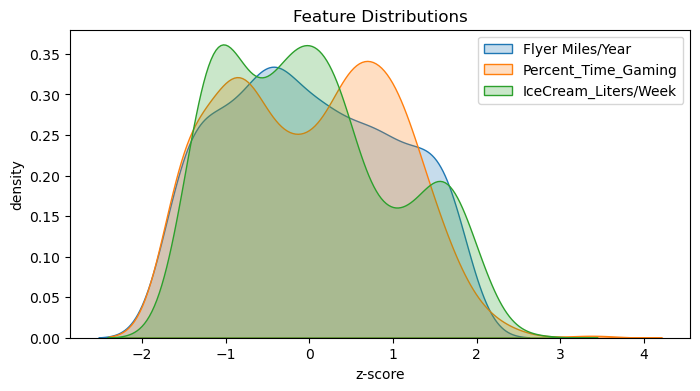
\includegraphics[width=0.65\textwidth, height=0.25\textheight]{pre_a.png}
        \caption{\small{Standardized Distributions}}
    \end{figure}
    \begin{figure}[H]
        \centering
        \begin{minipage}[t]{0.47\textwidth}
            \centering
            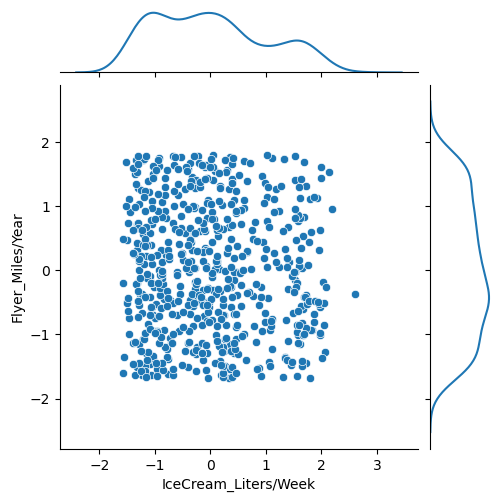
\includegraphics[width=\textwidth, height=0.3\textheight]{pre_c.png}
            \caption{\small{Flyer Miles/Year vs Ice Cream Liters/week}}
        \end{minipage}
        \hfill
        \begin{minipage}[t]{0.47\textwidth}
            \centering
            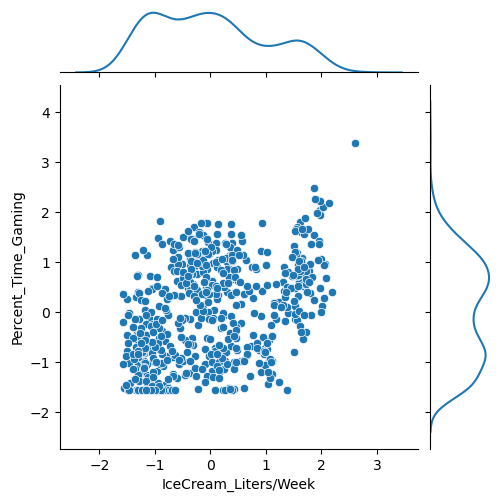
\includegraphics[width=\textwidth, height=0.3\textheight]{pre_b.png}
            \caption{\small{Percentage Time Gaming vs Ice Cream Liters/week}}
        \end{minipage}
    \end{figure}
    \begin{figure}[H]
        \centering
        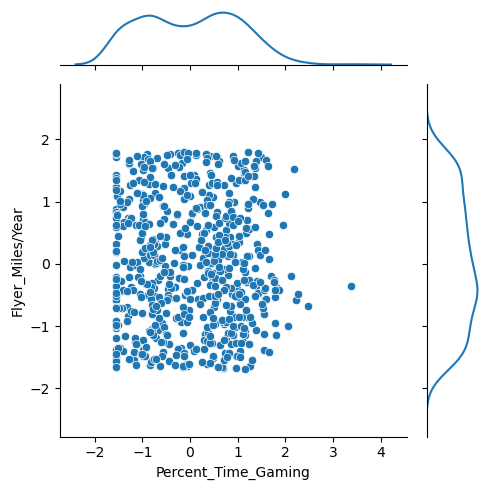
\includegraphics[width=0.47\textwidth, height=0.3\textheight]{pre_d.png}
        \caption{\small{Flyer Miles/Year vs Percentage Time Gaming}}
    \end{figure}

    We can also define a general cross validation helper function and store frequent performance
    metrics in a dictionary:

    \begin{figure}[H]
        \centering
        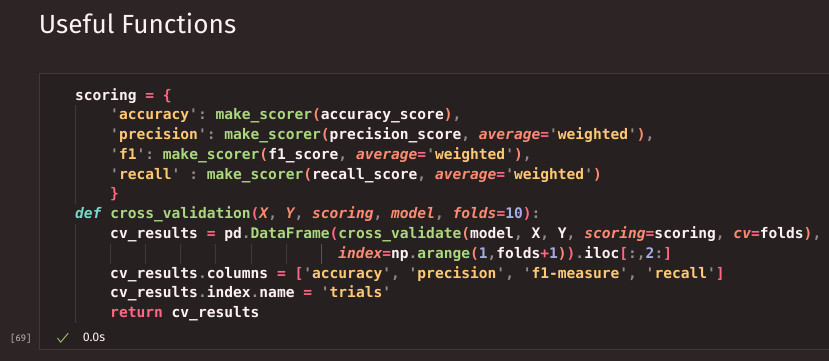
\includegraphics[width=0.75\textwidth, height=0.35\textheight]{helper.png}
        \caption{\small{Utility Functions}}
    \end{figure}

    The following analysis will involve model selection and validation using only
    the \textbf{training dataset}. We will conclude with a final evaluation
    and comparison of the selected models using the \textbf{test dataset}.

    \newpage

\section*{Naive Bayes Classification (Gaussian Distribution)}

    \subsection*{Validation}

    Although some correlation can be observed between \textbf{Percentage Time Gaming} and
    \textbf{Ice Cream Liters/week}, Gaussian Naive Bayes remains a robust classification method due to
    roughly normal feature distributions and week/nonexistent overall feature pair correlations indicating
    high degree of feature independence.

    \begin{figure}[H]
        \centering
        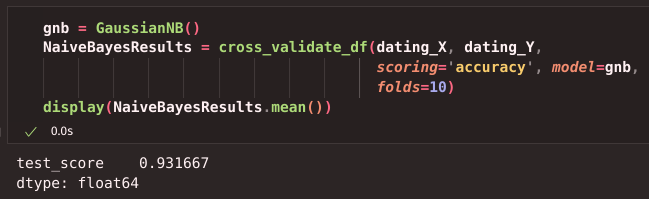
\includegraphics[width=0.75\textwidth, height=0.15\textheight]{NB_results.png}
        \caption{\small{Naive Bayes Cross Validation Results}}
    \end{figure}

\section*{K-NN Classification}

    \subsection*{Model Selection}

    The training data is shuffled for each of 100 repetitions during which we iterate through
    different k-values for k $\in [1,30]$, and calculate the corresponding test accuracy
    using 10-fold cross validation. We maintain a running total of the test accuracy for
    each model and then divide all accuracies by the number of repetitions (100) to get the
    mean accuracies. The final plot shows that $k=18$ has the highest accuracy, and so this
    is the model we select.
    
    \begin{figure}[H]
        \centering
        \begin{minipage}[t]{0.49\textwidth}
            \centering
            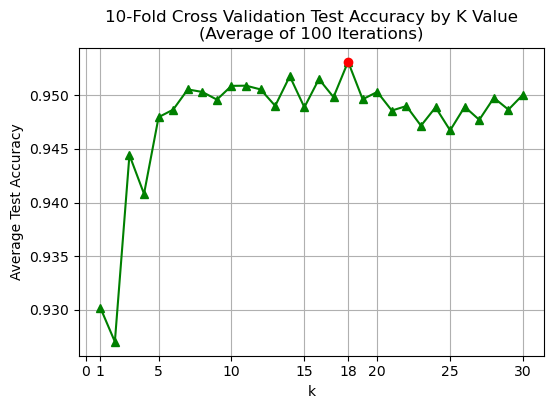
\includegraphics[width=\textwidth, height=0.25\textheight]{k-NN_selection.png}
            \caption{\small{Best K Hyperparameter Selection Plot}}
        \end{minipage}
        \hfill
        \begin{minipage}[t]{0.49\textwidth}
            \centering
            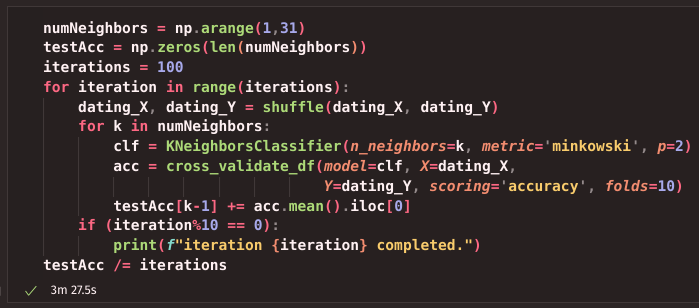
\includegraphics[width=\textwidth, height=0.17\textheight]{k-NN_selection_code.png}
            \caption{\small{Best K Hyperparameter Selection Code}}
        \end{minipage}
    \end{figure}

    \newpage

\section*{Decision Tree Classification}

    \subsection*{Model Selection}

    Using a similar approach to K-NN classification, we begin by shuffling the training data
    for each of the 100 repetitions. We then iterate over a range of maximum tree depths,
    creating decision trees using both entropy and Gini impurity measures. For each tree,
    10-fold cross-validation is applied to obtain accuracy scores, which are accumulated
    across repetitions for each depth and impurity measure. After completing all repetitions,
    the total accuracy scores are averaged by dividing by the number of repetitions,
    yielding the mean accuracy for each depth. Finally, we plot the average accuracies
    by depth for both impurity measures, allowing us to identify the optimal parameters for
    the decision tree model.

    \begin{figure}[H]
        \centering
        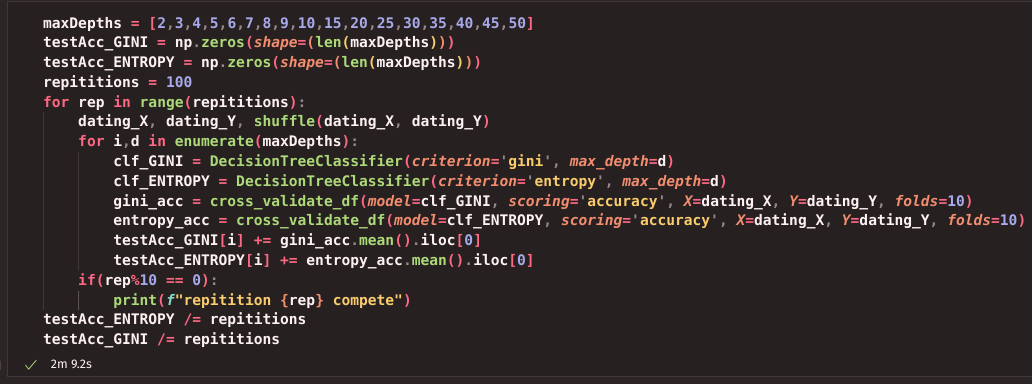
\includegraphics[width=0.7\textwidth, height=0.18\textheight]{tree_selection_code.png}
        \caption{\small{Decision Tree Model Selection Code}}
    \end{figure}
    \begin{figure}[H]
        \centering
        \begin{minipage}[t]{0.49\textwidth}
            \centering
            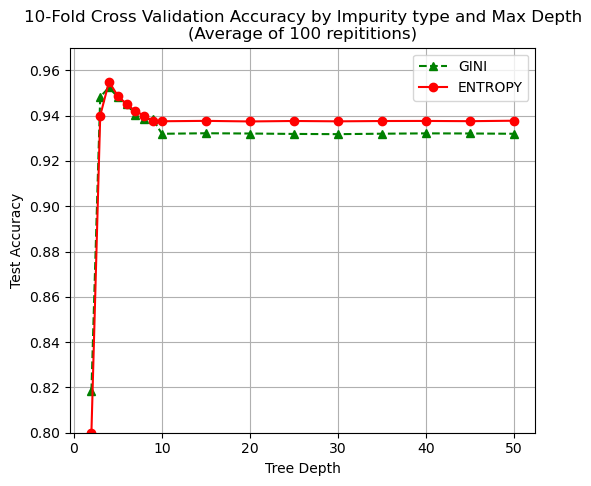
\includegraphics[width=\textwidth, height=0.25\textheight]{tree_selection1.png}
            \caption{\small{Accuracy by Impurity Measure and Depth}}
        \end{minipage}
        \hfill
        \begin{minipage}[t]{0.49\textwidth}
            \centering
            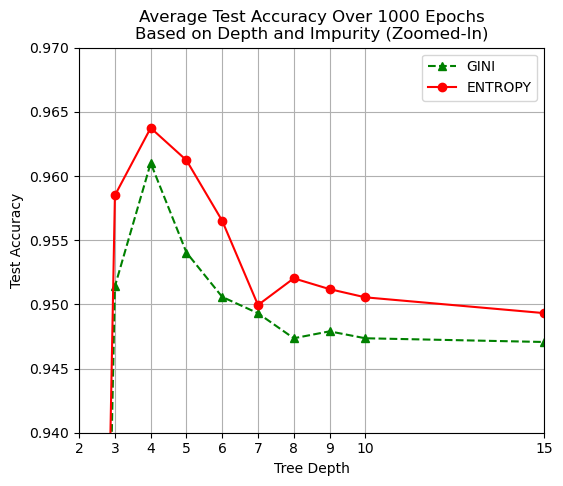
\includegraphics[width=\textwidth, height=0.25\textheight]{tree_selection2.png}
            \caption{\small{Accuracy by Impurity Measure and Depth (Zoomed-In)}}
        \end{minipage}
    \end{figure}

    We can see that a max depth of 4 and the entropy impurity measure yields the best
    performing decision tree model. 

    \newpage

\section*{Test Set Validation}

    \subsection*{Validation}

    After having selected and trained the best models on the training dataset, we can now
    make classification predictions on the unseen instances from the test dataset.

    \begin{figure}[H]
        \centering
        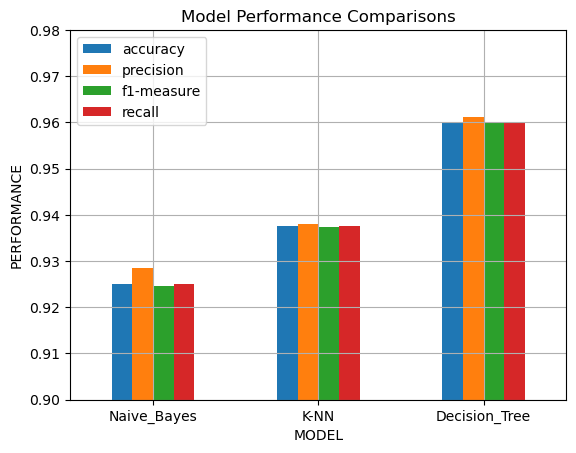
\includegraphics[width=0.7\textwidth, height=0.4\textheight]{comparison.png}
        \caption{\small{Model Comparison Plot}}
    \end{figure}
    \begin{figure}[H]
        \centering
        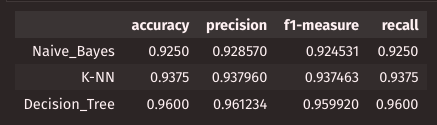
\includegraphics[width=0.7\textwidth, height=0.15\textheight]{comparison_table.png}
        \caption{\small{Model Comparison Table}}
    \end{figure}

    In conclusion, a decision tree using entropy impurity and a maximum tree depth of 4
    is the best model for predicting the degree to which the customer will like a given
    person based on the provided features.


\end{document}